\section{Probabilistische Turingmaschinen}
\subsection{Definition}
Wir nutzen das Modell der Mehrband-Turingmaschine um abstrakt die Fähigkeit einer Turing-Maschine zu zeigen, eine zufällige Auswahl zu treffen, entsprechend einem Programm, das einen Zufallszahlengenerator einmal oder mehrfach aufruft.
Auf dem ersten Band steht wie bei einer Mehrband-Turingmaschine üblich die Eingabe.
Das zweite Band, das sogenannte \emph{Zufallsband}, ist vollständig mit den Symbolen $1$ und $0$, die zufällig und unabhängig voneinander mit der Wahrscheinlichkeit $Pr[x] = \frac{1}{2}, x \in \{0, 1\}$.
Die übrigen Bänder sind initial leer und können nach Bedarf als \emph{Hilfsbänder} genutzt werden.

\begin{figure}[h]
	\centering
	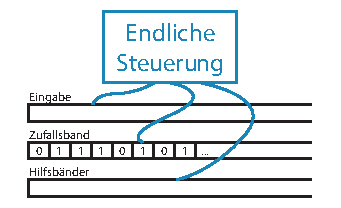
\includegraphics[width=.8\textwidth]{Graphics/Probabilistic_TM}	
	\caption{Darstellung einer zufallsabhängigen Turingmaschine}
	\label{fig:probabilistic_tm}
\end{figure}

Wir nennen dieses Modell einer Turingmaschine \emph{zufallsabhängige Turingmaschine} oder \emph{probabilistische Turingmaschine}.

\paragraph{Bemerkung}
Eine zufallsabhängige Turingmaschine kann als eine Art nichtdeterministische Turingmaschine gesehen werden, bei welcher jeder nichtdeterministische Berechnungsschritt vom Inhalt des Zufallsbandes abhängt.
Einen solchen Berechnungsschritt bezeichnen wir im Folgenden als \emph{Coin-Flip-Schritt}.


\subsection{Initialisierung des Zufallsbandes}
\paragraph{Beobachtung:}
Da die komplette Initialisierung des unendlichen Zufallsbandes mit den Symbolen $1$ und $0$ ist nicht realistisch, da diese nie terminiert.

\paragraph{Lösung:}
Das Zufallsband ist initial ebenfalls leer, enthält also nur \emph{Blanks}. 
Liest der Lese-Schreibkopf auf dem Zufallsband nun ein \emph{Blank}, so wird intern mittels eines Zufallsgenerators eine $1$ oder eine $0$ erzeugt und auf das Zufallsband geschrieben.
Das generierte Symbol wird anschließend nicht wieder verändert.
Auf diese Weise scheint das Zufallsband vollständig initialisiert.


\subsection{Sprache einer zufallsabhängigen Turingmaschine}
Wir sind an Berechnungsmodelle gewöhnt, die immer eine Sprache akzeptieren, zum Beispiel auch $\emptyset$ oder $\Sigma^*$.
Mit dem Begriff der \emph{Akzeptanz} müssen wir bei einer zufallsabhängigen Turingmaschine $M$ etwas vorsichtiger umgehen.
So kann es zum Beispiel vorkommen, dass gar keine Sprache akzeptiert wird.
Es ist sogar möglich, dass $M$ bei gleicher Eingabe und entsprechendem Inhalt auf dem Zufallsband akzeptiert und bei einem anderen Inhalt auf dem Zufallsband nicht akzeptiert.
Dieses Verhalten ist eventuell sogar gewünscht, wenn eine zufallsabhängige Turingmaschine effizienter arbeiten soll als eine deterministische.

Wollen wir eine Aussage über die Verarbeitung einer Eingabe $w$ auf einer zufallsabhängigen Turingmaschine $M$ machen, so müssen wir betrachten wie $M$ sich bei allen möglichen Inhalten des Zufallsbandes verhält.

\paragraph{Definition}
Sei $M$ eine zufallsabhängige Turingmaschine.
Für die Wahrscheinlichkeit einer Berechnung $b$ auf einer Eingabe $w$ gilt
\begin{equation*}
	Pr[b] = 2^{-k}
\end{equation*}
wobei $k$ die Anzahl der \emph{Coin-Flip-Schritte} in $b$ ist. 
Ferner gilt für die Akzeptanz von $w$
\begin{equation*}
	Pr[M\ akzeptiert\ w] = \sum_{\substack{b\ ist\ akz.\\ Berechnung}} Pr[b] 
\end{equation*}

\subsection{Beispiel}
\label{PTM_Example1}
Die folgende Tabelle beschreibt die Übergangsfunktion einer zufallsabhängigen Turingmaschine $M$ mit dem Eingabealphabet $\Sigma = \{a, b\}$, wobei gilt
\begin{description}
	\item [$\boldsymbol{q_i}$] in der Beschriftung der Zeilen bezeichnet einen Zustand mit $q_i \in Q$,
	\item [$\boldsymbol{\rightarrow q_0}$] bezeichnet den Startzustand $q_0 \in Q$,
	\item [$*\boldsymbol{q_i}$] bezeichnet einen Endzustand $q_i \in F$,
	\item [XY] in der Beschriftung der Spalten bezeichnen die gelesenen Symbole auf dem Eingabeband ($X$) und auf dem Zufallsband ($Y$),
	\item [qUVDE] in einer Zelle bedeutet, dass $M$ in den Zustand $q$ wechselt, $U$ auf das Eingabe- und $V$ auf das Zufallsband schreibt und den Eingabekopf in Richtung $D$ sowie den Kopf auf dem Zufallsband in Richtung $E$ bewegt,
	\item [S] als Richtung bedeutet, dass der Kopf auf der aktuellen Position stehen bleibt,
	\item [R] als Richtung bedeutet, dass der Kopf nach rechts bewegt wird.
\end{description}

\bgroup
	\def\arraystretch{1.5}
	\begin{tabular}{r || c | c | c | c | c | c}
		& \textbf{a0} & \textbf{a1} & \textbf{b0} & \textbf{b1} & \textbf{B0} & \textbf{B1} \\
		\hline \hline
		$\boldsymbol{\rightarrow q_0}$ & $q_1a0RS$ & $q_3a1SR$ & $q_2b0RS$ & $q_3b1SR$ & & \\
		\hline
		$\boldsymbol{q_1}$ & $q_1a0RS$ & & & & $q_4B0SS$ & \\
		\hline
		$\boldsymbol{q_2}$ & & & $q_2b0RS$ & & $q_4B0SS$ & \\
		\hline
		$\boldsymbol{q_3}$ & $q_3a0RR$ & & & $q_3b1RR$ & $q_4B0SS$ & $q_4B1SS$ \\
		\hline
		$\boldsymbol{*q_4}$ & & & & & & \\
	\end{tabular}
\egroup

\begin{description}
	\item [a.)] Wie könnte sich $M$ auf der Eingabe $w = ab$ verhalten?
	\item [b.)] Mit welcher Wahrscheinlichkeit akzeptiert $M$ eine homogene Eingabe $a^i,\ i \in \mathbb{N}^+$?
	\item [c.)] Mit welcher Wahrscheinlichkeit akzeptiert $M$ eine heterogene Eingabe? Berechnen Sie $P(M\ akzeptiert\ w),\ w = aabab$! 
\end{description}

\paragraph{Lösungen:}
\begin{description}
	\item [a.)] \ \\
\begin{tikzpicture}[level/.style={sibling distance=4cm/#1}]
	\node (0)[circle,draw]{$q_0$}
  	child {
  		node (12)[circle,draw]{$q_1$} 
  		child {
  			node (21)[circle,draw]{$\times$}
  			edge from parent node[left,draw=none,myblue] {$b0$}
  		}
  		child {
  			node (22)[circle,draw]{$\times$}
  			edge from parent node[right,draw=none,myblue] {$b1$}
  		}
  		edge from parent node[left,draw=none,myblue] {$a0$}
    }
    child {
    	node (11)[circle,draw]{$q_3$}
    	child {
  			node (23)[circle,draw]{$\times$}
  			edge from parent node[left,draw=none,myblue] {$b0$}
  		}
  		child {
  			node (24)[circle,draw]{$q_3$}
  			child {
  				node (31)[circle,draw]{$\checkmark$}
  				edge from parent node[left,draw=none,myblue] {$B0$}
  			}
  			child {
  				node (32)[circle,draw]{$\checkmark$}
  				edge from parent node[right,draw=none,myblue] {$B1$}
  			}
  			edge from parent node[right,draw=none,myblue] {$b1$}
  		}
  		edge from parent node[right,draw=none,myblue] {$a1$}
    };
\end{tikzpicture}
	\item [b.)] $\underbrace{\frac{1}{2}}_{\substack{1.\ Zufallsbit \\ ist\ 0}}\ +\ \underbrace{\frac{1}{2}2^{-i}}_{\substack{1.\ Zufallsbit \\ ist\ 1}} \quad = \quad \frac{1}{2} + 2^{-(i+1)}$
	\item [c.)] $\underbrace{0}_{\substack{1.\ Zufallsbit \\ ist\ 0}}\ +\ \underbrace{\frac{1}{2}2^{-i}}_{\substack{1.\ Zufallsbit \\ ist\ 1}} \quad = \quad 2^{-(i+1)}$ \\ $\Rightarrow\ Pr[M\ akzeptiert\ w]\ =\ 2^{-6}\ =\ \frac{1}{64}$
\end{description}



